
\section{Results}
\begin{figure}
  \setlength{\unitlength}{\textwidth}
  \begin{picture}(1,0.72)
%(0,0.35)
    
    % % %Parkinson Data 
    \put(0.025,0.48){\includegraphics[width=0.5\unitlength]{../FnP/gnuplot/displacement_amp_re_parkinson_1.eps}}
    \put(0.025,0.25){\includegraphics[width=0.5\unitlength]{../FnP/gnuplot/velocity_amp_re_parkinson.eps}}
    \put(0.025,0.02){\includegraphics[width=0.5\unitlength]{../FnP/gnuplot/mean_power_re_parkinson.eps}}
    
    % Re 165 Data 
    \put(0.495,0.48){\includegraphics[width=0.5\unitlength]{../FnP/gnuplot/displacement_amp_re165.eps}}
    \put(0.495,0.25){\includegraphics[width=0.5\unitlength]{../FnP/gnuplot/velocity_amp_re165.eps}}
    \put(0.495,0.02){\includegraphics[width=0.5\unitlength]{../FnP/gnuplot/mean_power_re_165.eps}}
   
%    \put(0.25,0.93){\ustar}
%    \put(0.8,0.93){\ustar}
%    \put(0.25,0.63){\ustar}
%   \put(0.8,0.63){\ustar}
    \put(0.25,0.0){\ustar}
    \put(0.75,0.0){\ustar}
    
    \put(0.00,0.685){$\frac{A}{D}$}
%    \put(0.52,1.075){$\frac{A}{D}$}
    \put(0.00,0.44){$\frac{V}{D}$}
%    \put(0.52,0.83){$\frac{V}{D}$}
    \put(-0.01,0.15){$\frac{P_{m}}{\rho \mathcal{A}U^3 }$}
%    \put(0.5,0.54){$\frac{P_{m}}{\rho \mathcal{A}U^3 }$}
    
    \put(0.095,0.685){\small(a)}
    \put(0.555,0.685){\small(b)}
    \put(0.095,0.455){\small(c)}
    \put(0.555,0.455){\small(d)}
    \put(0.095,0.225){\small(e)}
    \put(0.555,0.225){\small(f)}   
  \end{picture}

%  \vspace{-4cm}
  \caption{Velocity and displacement amplitude and mean power  as a function of $U^*$. (a), (c) and (e) are calculated using input $C_y$ data at Re=22300 obtained by \cite{Parkinson1964} and present data at three different damping ratios: $\zeta=0.0125$ (\ding{83}), $\zeta=0.015$ (\ding{116}) and $\zeta=0.0175$ (\ding{108}). (b),(d) and (f) are from $C_y$ data at Re=165 and are calculated  from the fixed body simulations and present data at three different  different damping ratios: $\zeta=0.075$ ($\times$), $\zeta=0.1$ (\ding{117}) and $\zeta=0.15$ (+). The multiple branches for the higher Re are due to the hysteresis between two solutions.}
  
  \label{fig:uncollapsed_data}
\end{figure}



\subsection{Displacement,velocity and power output as a function of reduced velocity}


 The quasi-steady analysis data reveals that the displacement amplitude tend to grow with increasing $U^*$ Fig.\ref{fig:Displacement_amplitude}. The onset of galloping is delayed with increasing $\zeta$.  !!! State how this is consistent with previous studies by Parkinson and a few other key studies. Also state that this is observed for both low and high RE cases. Also point out that hystersis is observed for the high Re case and not in the low Re case. This is also consistant with earlier studies which you should point out.
 
 \subsubsection*{Power vs $U^*$}
 
 The mean power grows, peaks and then reduces as $U^*$ is increased Fig.\ref{fig:uncollapsed_data} (e) and (f) for each value of $\zeta$. A shift of the peak power could be observed as $\zeta$ increases. However, the magnitude of the peaks remain constant for all the values of $\zeta$. A similar observation could be made from the results of \cite{Barrero-Gil2010a}. It could be observed that unlike VIV the  system has no preferred frequency. The onset of galloping and the peak power occurs at different $U^*$ at when the damping ratio is changed. The peak power remains constant regardless of $U^*$.
 
 \subsection{Galloping response and natural frequency}
 
 If the oscillator equation Eq.\eqref{final_equation_motion} is considered from a power perspective (disregarding the shedding term as the net effect is negligible !!! this should be elaborated further possibly in an earlier section as to why. I suggest when you talk about the shedding inputs and discuss the findings from Joel. Only negligible when system oscillates at natural frequency which is far from shedding frequency), it could be seen that the forcing term on RHS of the equation is only dependent on transverse velocity($\dot{y}$) which is essentially the input power of the system. On the RHS, the mechanical damping or system damping is the only term that takes out power at any instant by the product of damping force and the velocity ($P_d$). The inertia and the stiffness terms governs the frequency of the system but the forces associated by those terms are conservative forces i.e there is zero net energy in or out of the system when averaged over a period. Therefore it appears that the system is governed by the transverse velocity rather than the natural frequency.
 

 Using $U^*$ and $\zeta$ assumes that the system has a preferred frequency. The effect of fixing $\zeta$ and increasing $U^*$ actually decreases damping constant for a fixed free-stream velocity.($U^*=\frac{U}{f \times D}$, $\zeta= \frac{c}{2 m \omega_n}$ ). Both these effects leads to the multiple lines that horizontally transpose when $\zeta$ is increased(Fig.\ref{fig:mean_power}). Therefore the effect of $\zeta$ essentially scales up the damping coefficient for a fixed $U$. 
 \vspace{1cm}
 
 Therefore a single set of results for a given $a_1,a_3, a_5$ and $a_7$ could be obtained if we were to plot displacement, velocity and power as a function of damping constant $c$ (Fig \ref{fig:velocity_collapsed}, \ref{fig:meanpower_collapsed}). A similar maximum velocity could be obtained for a given `c'. Fig.\ref{fig:same_max_vel} clearly shows the validity of this argument. 

\begin{figure}
  \setlength{\unitlength}{\textwidth}
       
        \begin{picture}(1,0.52)

      % % % Parkinson Data 
      \put(0.025,0.27){\includegraphics[width=0.5\unitlength]{../FnP/gnuplot/velocity_amp_collapsed_parkinson.eps}}
      \put(0.495,0.27){\includegraphics[width=0.5\unitlength]{../FnP/gnuplot/velocity_amp_collapsed_re165.eps}}
      
      \put(0.025,0.02){\includegraphics[width=0.5\unitlength]{../FnP/gnuplot/mean_power_collapsed_parkinson.eps}}
      \put(0.495,0.02){\includegraphics[width=0.5\unitlength]{../FnP/gnuplot/mean_power_collapsed_re_165.eps}}
      
      
      \put(0.23,0.00){ $c\rho\mathcal{A}U$}
      \put(0.73,0.00){ $c\rho\mathcal{A}U$}
      
      \put(0.01,0.405){$\frac{V}{D}$}
      
      \put(0,0.13){$\frac{P_{m}}{\rho \mathcal{A}U^3 }$}
      \put(0.085,0.475){\small(a)}
      \put(0.555,0.475){\small(b)}
      \put(0.095,0.225){\small(c)}
      \put(0.555,0.225){\small(d)}
      
    \end{picture}

  \caption{ Velocity amplitude and mean power  as a function of $c$ (damping constant). (a) and (c)  are calculated using input $C_y$ data at Re=22300 obtained by \cite{Parkinson1964} and present data at three different damping ratios: $\zeta=0.0125$ (\ding{83}), $\zeta=0.015$ (\ding{116}) and $\zeta=0.0175$ (\ding{108}). (b)and (d)  are at Re=165 are calculated  from the fixed body simulations and present data from three different damping ratios: $\zeta=0.075$ ($\times$), $\zeta=0.1$ (\ding{117}) and $\zeta=0.15$ (+). The collapsed data implies that there is no frequency selection and the tuning parameter of the mechanical side of the system is the damping constant to obtain an optimum power output.}
    \label{fig:collpased_data}
\end{figure}

\ %vspace{10cm}

 
 \begin{figure}[h!]
 \begin{subfigure}[b]{0.5\textwidth}
 \centering
 \label{fig:u_60_zet_0075}
 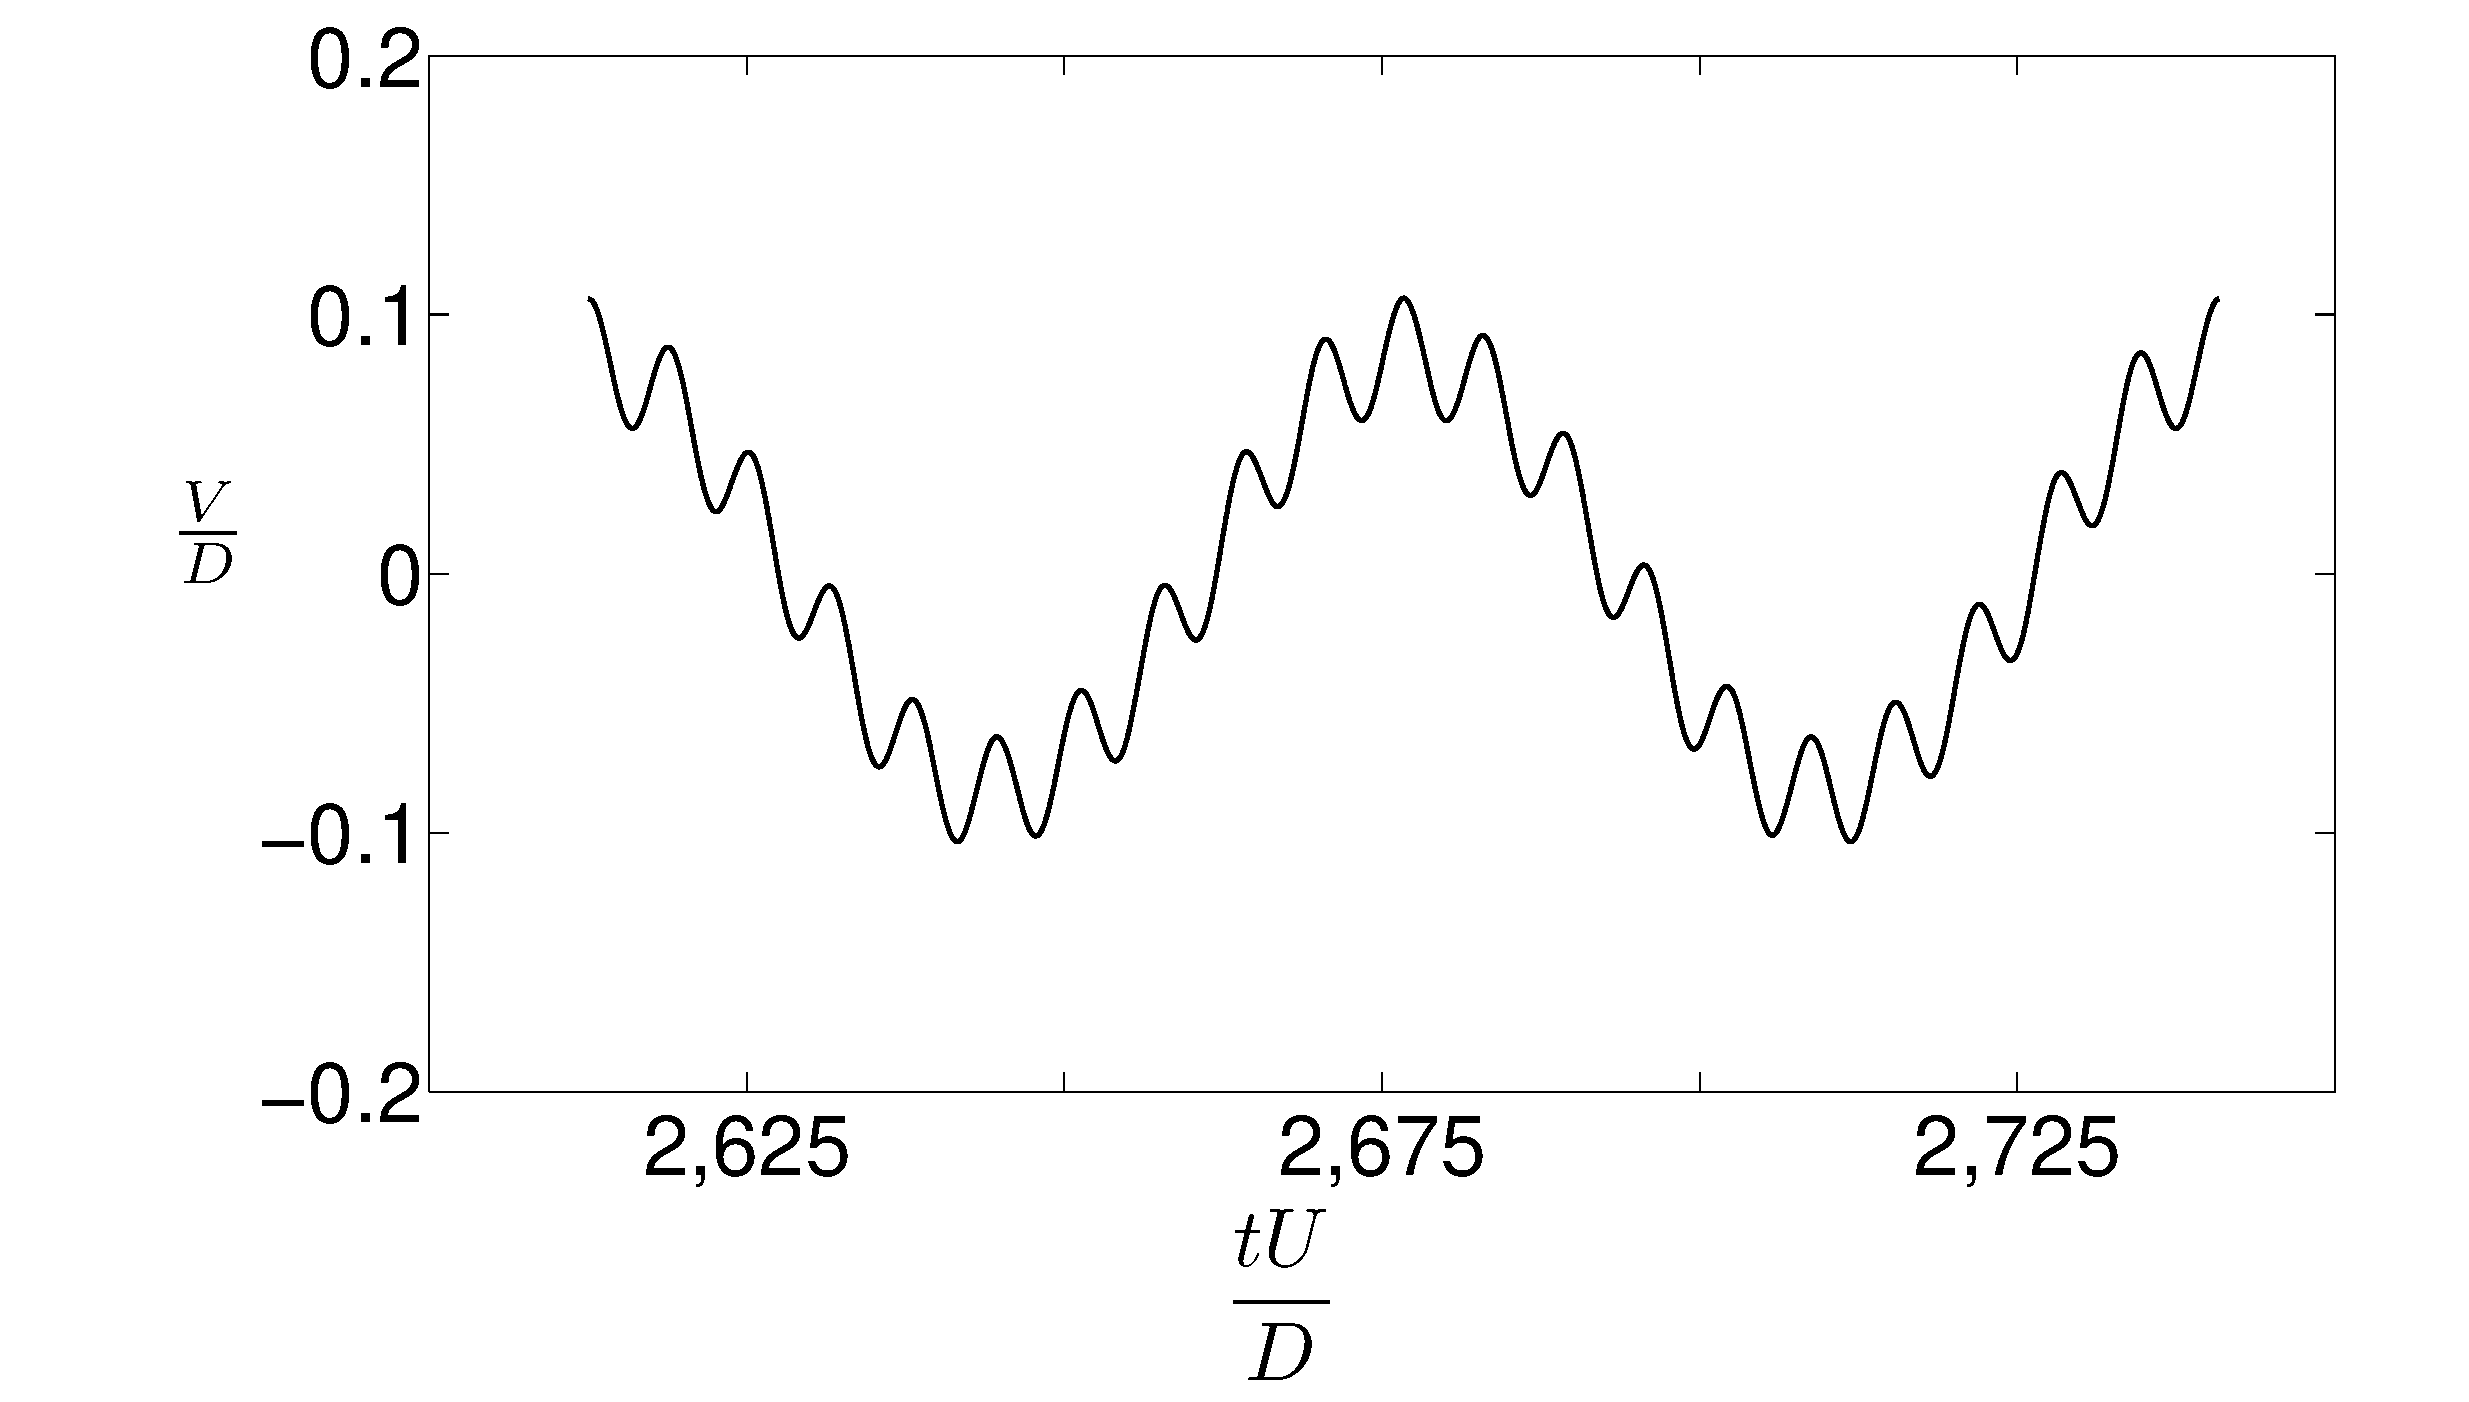
\includegraphics[width=\textwidth]{../FnP/latest/u_60_zet_0075}
 \caption{}
 \end{subfigure}
 
 \begin{subfigure}[b]{0.5\textwidth}
 \centering
 \label{fig:u_150_zet_017}
 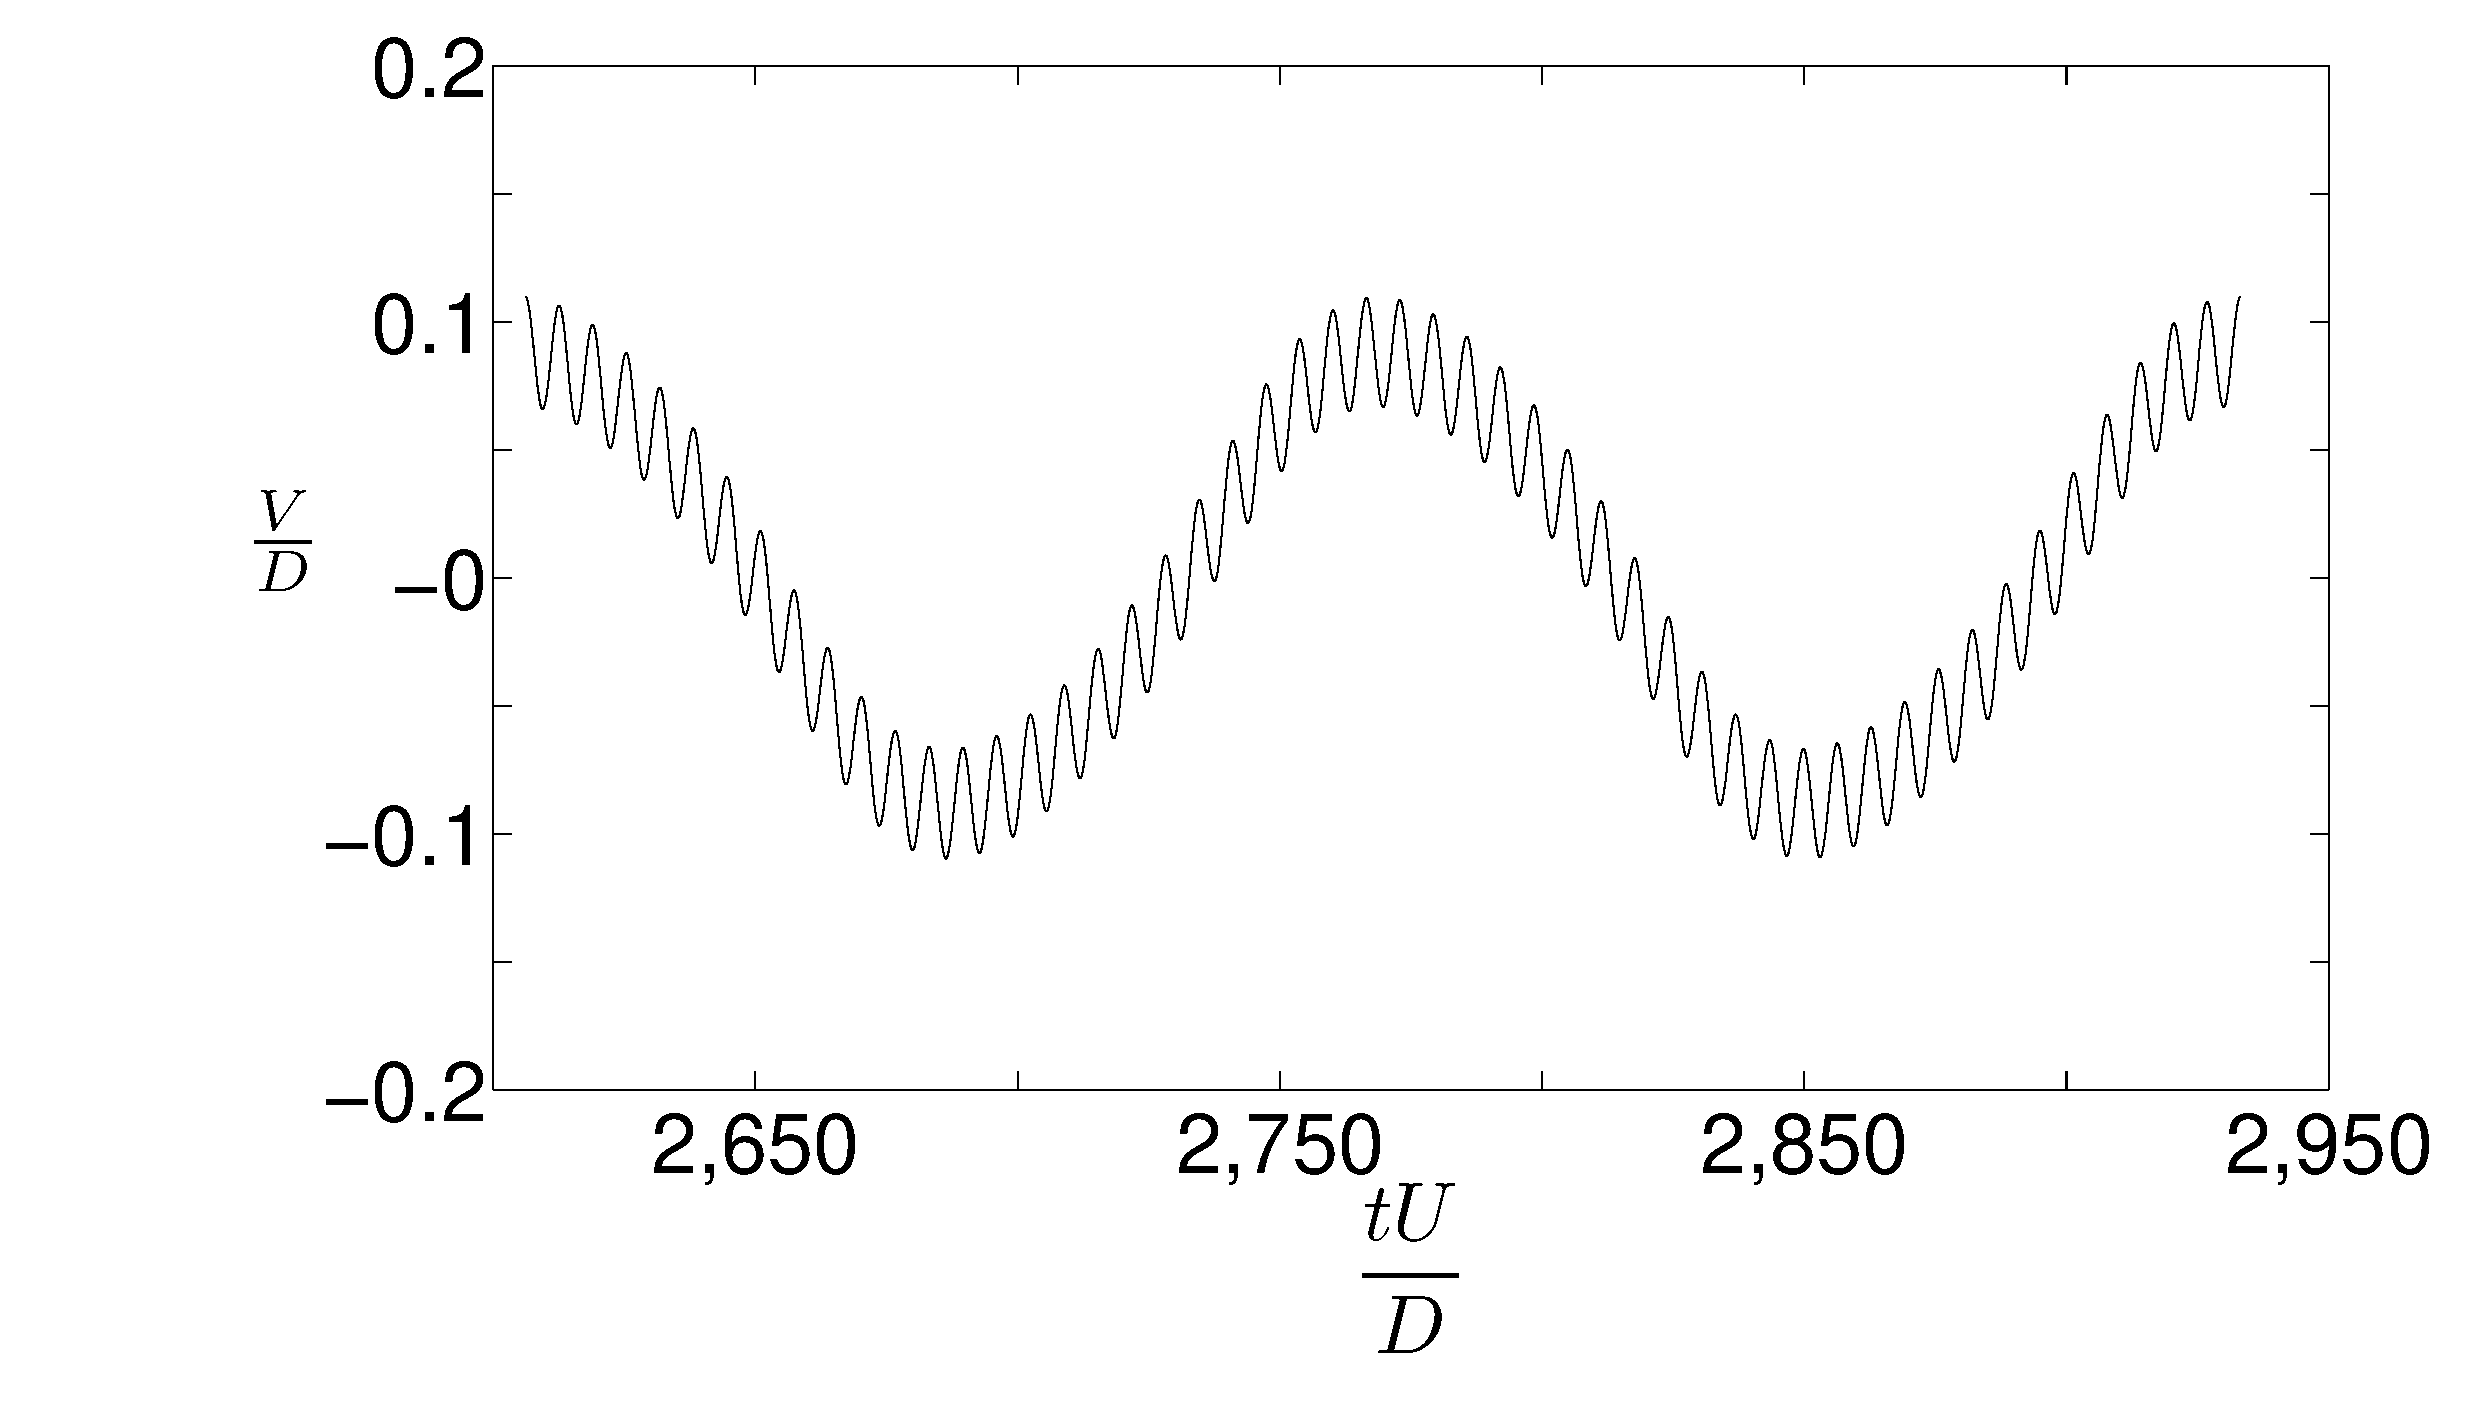
\includegraphics[width=\textwidth]{../FnP/latest/u_150_zet_0175}
 \caption{}
 \end{subfigure}
 \caption{Comparison of time histories of velocity at the same damping ratio $c=0.12$ at different $U^*$. Sub-figure (a) represents data at $U^*=60$ $\zeta=0.075$ and sub-figure (b) represents data at $U^*=150$ $\zeta=0.0175$ at Re 165 }
 \label{fig:same_max_vel}
 \end{figure}
 
 
 
 
 
 Power could be expressed as the product of force and velocity. Therefore the transferred power form fluid-to-body could be expressed as $P_t=F_y\dot{y}$. Similarly the dissipated power due to the mechanical damping could be expressed as $P_d=(c\dot{y})\dot{y}.$

The analysis of time histories of $P_t $ and $P_d$ at key regions (Fig.\ref{fig:regions_1}) on the mean power vs $U^*$ provides an detailed explanation on what exactly happens to power when the reduced velocity is increased. It has been established earlier that the damping factor is a function of $U^*$. It could be derived that $U^*$ is inversely proportional to damping coefficient. 

\begin{figure}[h!]
\centering
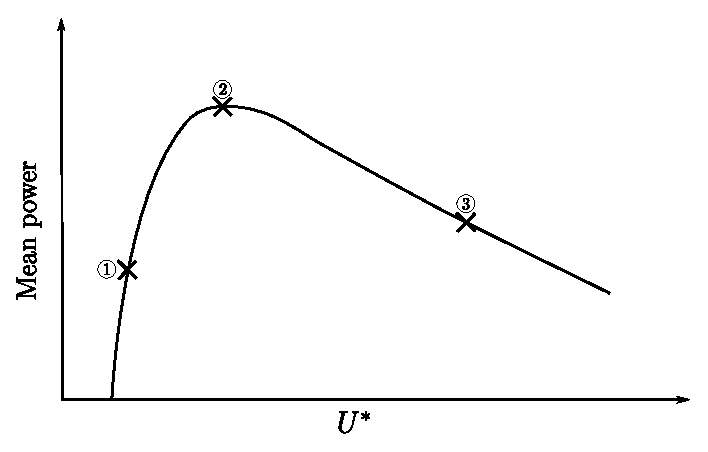
\includegraphics[width=0.5\textwidth]{../FnP/sketch_1}
\caption{ Three key regions taken into account to analyse the time histories of power in a typical the Mean power vs. $U^*$ curve at Re 165 }
\label{fig:regions_1}
\end{figure}



\begin{figure}

  \setlength{\unitlength}{\textwidth}
 % \fbox{
  \begin{picture}(1,0.6)(0,0.35)
    
    % % %90
      \put(0.03,0.78){\includegraphics[width=0.35\unitlength]{../FnP/gnuplot/power_time_history_90.eps}}
      \put(0.03,.58){\includegraphics[width=0.35\unitlength]{../FnP/gnuplot/f_y_history_90.eps}}
      \put(0.03,0.4){\includegraphics[width=0.35\unitlength]{../FnP/gnuplot/theta_time_history_90.eps}}
      
      % %165
       \put(0.36,0.78){\includegraphics[width=0.35\unitlength]{../FnP/gnuplot/power_time_history_165.eps}}
       \put(0.36,.58){\includegraphics[width=0.35\unitlength]{../FnP/gnuplot/f_y_history_165.eps}}
       \put(0.36,0.4){\includegraphics[width=0.35\unitlength]{../FnP/gnuplot/theta_time_history_165.eps}}
       
       \put(0.68,0.78){\includegraphics[width=0.35\unitlength]{../FnP/gnuplot/power_time_history_400.eps}}
       \put(0.68,.58){\includegraphics[width=0.35\unitlength]{../FnP/gnuplot/f_y_history_400.eps}}
       \put(0.68,0.4){\includegraphics[width=0.35\unitlength]{../FnP/gnuplot/theta_time_history_400.eps}}
      
            
      
      
   
 	\put(0.55,0.36){\large $\frac{tU}{D}$}
 	\put(0.2,0.36){\large $\frac{tU}{D}$}
    \put(0.85,0.36){\large $\frac{tU}{D}$}
    
   
   	
   	\put(0.0,0.87){$\frac{P}{\rho \mathcal{A}U^3}$}
    \put(0.01,0.66){$F_y$}
    \put(0.01,0.49){$\theta$}
   	

    \put(0.08,0.78){(a)}
    \put(0.08,0.58){(d)}
    \put(0.08,0.38){(g)}
    
    \put(0.4,0.78){(b)}
    \put(0.4,0.58){(e)}
    \put(0.4,0.38){(h)}
    
    \put(0.72,0.78){(c)}
    \put(0.72,0.58){(f)}
    \put(0.72,0.38){(i)}
       
  \end{picture}
%}
  \caption{Time histories of $P_t$,$P_d$,$F_y$ and $\theta$ at $\ustar=90,165$ and $400$ where the mean power dissipated due to mechanical was calculated using equation \hilight{equation}. Data was obtained at $\zeta=0.1$ and $m^*=40$. The time histories of $P_t$ ( \solidrule[4mm]\hspace{1mm}) and $P_d$ (\protect\dashedrule) are presented in (a), (b) and (c) where \ustar is 90, 165 and 400 respectively.(d), (e) and (f) shows time histories of the instantaneous force $F_y$ and (g), (h) and (i) shows the time history of the instantaneous angle $\theta$ of the corresponding power plots above}
    \label{fig:power_time_histories}
\end{figure}










At region 3 ($U^*= 400$) `$c$' is significantly low therefore the mean power output is less. From Fig. \ref{fig:power_time_hostory_u_400fig} it could be observed that $P_t$ becomes negative. This is due to the fact that $\theta$ moves to a region where $F_y$ becomes negative while velocity is positive. Hence $P_t$ becomes positive. On the other hand in terms of an energy point  of view, the mechanical damping is not sufficient to dissipate out the total transferred energy (as `$c$' is substantially low), therefore  part of it  is transferred back to the fluid. At region 2 where the  mean power becomes maximum($U=165$), $P_t$ does not become a pure sinusoidal signal. However, the  signal remains periodic. From the time history graph of $P_t$ two `peaks' are present in a single half cycle (Fig \ref{fig:power_time_hostory_u_165}). From  Fig. \ref{fig:F_theta_history_u_165} and \ref{fig:lift_theta} it could be observed that $\theta$ passes critical angle where the maximum $C_y$ is produced. Therefore, the force $F_y$ and $P_t$ reduces as the velocity increases. As the velocity $\dot{y}$ is sinusoidal $\theta$ recovers back and leading to two `peaks'  in a single half cycle.  $U^*=90$ (region 1) the damping constant is high and therefore a clear sinusoidal signal could be observed for both $P_d$ and $P_t$ Fig. \ref{fig:power_time_hostory_u_90}. From Fig. \ref{fig:lift_theta} and  \ref{fig:F_theta_history_u_90fig}  it is possible to see that the $\theta$  does not exceed the critical angle where the maximum $C_y$ (and therefore maximum $F_y$ ) is produced. Hence both $P_d$ and $P_t$ becomes sinusoidal.
  
  
  \begin{figure}
\centering
\includegraphics[width=0.8\textwidth]{../FnP/gnuplot/mean_power_collapsed_mstar}
\caption{$m^*=10$ (\ding{108}), $m^*=20$ ( \ding{83}),  $m^*=40$ (\ding{115}) and   $m^* = 60$ ($+$)}
\label{fig:mean_power_collapsed_mstar}
\end{figure}

  
  


\subsection{Effect of $m^*$}

%\begin{figure}
%\centering
%\includegraphics[width=0.8\textwidth]{../gnuplot/mean_power_collapsed_mstar.eps}
%\caption{Collapsed normalised mean power as a function of damping constant `$c$' at different $m^*$  ,  $m^*=10$ (\ding{108}), $m^*=20$ ( \ding{83}),  $m^*=30$ (\ding{115}),  $m^*=40$  ($\times$)and   $m^* = 60$ ($\bigcirc$), Obtained using QSS assumption at  $\zeta=0.1$ and Re = 165) } 
%\label{fig:power_mstar_collapsed_165}
%\end{figure}

The maximum mean power at different  $m^*$ Fig.\ref{fig:power_mstar_collapsed_165} was constant beyond $m^*=30$. However, at $m^* \leq 30$ an effect of $m^*$ could be observed, where the maximum of the mean power curve reduced as $m^*$ was reduced. This may be due to the fact that shedding dominates as the inertia of the system is reduced. This was also reported by \cite{Joly2012} where an influence of vortex shedding was present on galloping amplitude at low mass ratios. 


\subsection{Comparsion with FSI simulations}
 Similar trends are captured for both displacement and velocity amplitudes between QSS and FSI simulations (Fig. \ref{fig:QSS_FSI_dis_amp} and \ref{fig:QSS_FSI_vel_amp}). Quantitatively a large discrepancy  could be observed between QSS and FSI data. Therefore the power also becomes significantly low. The reasoning behind this the fact is that galloping is weak at Re 165 and therefore fluid damping has a significant effect. It was reported by \cite{Barrero-Gil2009} that galloping occur ar Re $\geq 159$
 
\begin{figure}
  \setlength{\unitlength}{\textwidth}

  \begin{picture}(1,1.13)(0,0)
    
    % % %90
      \put(0.25,0.78){\includegraphics[width=0.5\unitlength]{../FnP/gnuplot/fsi_displacement.eps}}
      \put(0.25,0.4){\includegraphics[width=0.5\unitlength]{../FnP/gnuplot/fsi_velocity.eps}}
      \put(0.25,0.025){\includegraphics[width=0.5\unitlength]{../FnP/gnuplot/fsi_power.eps}}
     
   
	
            
      
      
   
 	\put(0.25,0.98){ \large $\frac{A}{D}$} 	
 	\put(0.25,0.62){\large $\frac{V}{D}$}
 	\put(0.2,0.23){\large $\frac{P_{m}}{\rho \mathcal{A}U^3 }$}
 	
% 	 	\put(0.25,0.88){ \ustar} 	
% 	 	\put(0.8,0.88){ \ustar}
 	 	\put(0.5,0.0){ \ustar}



    \put(0.36,1.1){(a)}
    \put(0.34,0.72){(b)}
    \put(0.34,0.34){(c)}
   
       

  \end{picture}  
	
  \caption{Comparison of QSS (\ding{83}) and FSI (\ding{108}) data of displacement amplitude, velocity amplitude and mean power as a function of \ustar represented by (a), (b) and (c)respectively. Data were obtained at Re=165 and $\zeta=0.075$. An average error of $34\%$ could be observed for both displacement and velocity amplitude. Essential physics i.e the rise and fall of mean power could be captured of the FSI data}
    \label{fig:FSI_QSS_compare}
\end{figure}

%\section{Conclusion}









 

 
 
 

 
 


 % % % % % % % % % % % % % % % % % % % % % % % % % % % % % % % % % % % % % % % % %

 
 
 
 
 
 
 
 
 
 
  
 
 